  \documentclass{llncs}
\usepackage{amsmath}
\usepackage{txfonts}
\usepackage[boxed]{algorithm2e}
\usepackage{amssymb}
\usepackage[pdftex]{graphicx}
\usepackage{enumerate}
\DeclareGraphicsExtensions{.jpg, .png, .mps, .bmp, .pdf}
\usepackage{epsfig}
\usepackage{subfigure}
\newtheorem{Definition}{Definition} 
\newtheorem{Example}{Example} 
\newtheorem{Theorem}{Theorem} 
\newtheorem{Proof}{Proof} 
\newcommand{\denselist}{\topsep 0pt \itemsep -4pt}
\newcommand{\tup}[1]{\langle #1 \rangle}
\newcommand{\vvec}[1]{\mathbf{#1}}
\newcommand{\join}{\bowtie}
\newcommand{\R}{\mathcal{R}}
\newcommand{\Q}{\mathcal{Q}}
\newcommand{\body}{{body}}
\newcommand{\head}{{head}}
\newcommand{\qrule}{:\!\!-}
\newcommand{\arc}{\text{arc}}
\newcommand{\Theory}[1]{T(#1)}
\newcommand{\mcdsat}{\textsc{McdSat}}
\newcommand{\minicon}{{MiniCon}}
\newcommand{\Omit}[1]{}
\newcommand{\citeX}[1]{\citeauthor{#1}~\citeyear{#1}}

\begin{document}
\allowdisplaybreaks
\title{Selecting the Maximum-Utility  Web Services  Using Circuits}
\author{Daniel Izquierdo \inst{1}  and Blai Bonet \inst{1}  and Mar\'{\i}a-Esther Vidal \inst{1}}

\institute{Universidad Sim\'on Bol\'{\i}var\\
                Caracas, Venezuela\\
                \{idaniel,bonet,mvidal\}ldc.usb.ve} \maketitle
\begin{abstract}
In Service Oriented Architectures (SOA), concrete services are described in terms of functionality   and QoS parameters, while software applications are specified as workflows of abstract services and non-functional criteria that establish the  application desirable functionality and  expected quality, respectively.  During workflow execution time,  abstract services  are rewritten 
with the concrete services  that meet the workflow  functional and non-functional restrictions. Since, service selection is done on-the-flight and the space of concrete services may be very large, efficiency and scalability are required.  In this paper we propose the {\it SsdSat} framework to efficiently solve the problem of service selection in presence of a large number of concrete services.
First, we use the Local As View approach to describe the functionality  of the concrete services in terms of views of abstract services, the quality as an overall utility function that combines the different QoS values that describe the service, and  workflows as  conjunctive queries on abstract services. Based on this representation, we 
model the problem of service selection as a known problem in the area of integration systems referred as query rewriting using views.  We encode the service selection problem as a propositional theory whose models correspond to the composition of the services that implement the abstract workflow and have the same cost as the corresponding composition; known relationships between d-DNNF theories and arithmetic circuits are exploited to provide an efficient and scalable solution.  We report on the performance of our proposed approach, and we observe that  {\it SsdSat}  efficiently scales up to large instances of the service selection problem.  
 
 
\end{abstract}                
\section{Introduction}
Under the umbrella of the Semantic Web and supported by Service Oriented architectures, the number of Web data sources and services has exploded during the last few years.  For example,  currently, the molecular biology databases
collection includes 1,170 databases~\cite{Galperin09}, that is
95 more than the previous year~\cite{Galperin2008} and 110 more than two years ago~\cite{Galperin2007};  tools
and services as well as the number of instances published by these resources, follow a similar progression~\cite{Benson07}. Thanks
to this wealth, users rely more on various
digital tasks such as data retrieval from public data sources and
data analysis with Web tools or services organized in
complex workflows.  

In order to design an application, users usually specify the functionality in terms of a workflow of abstract services, while the desirable quality  is defined by restricting the values of the QoS parameters that describe the concrete available services. To evaluate the proposed workflow,  abstract services are instantiated on concrete services in a way restrictions on the QoS parameters are satisfied.  However, since the number of available sources has an impact on the performance of this task, techniques that enable us to efficiently scale up to a large number of services are required. 

In this paper we aim to provide a solution to this problem and provide techniques that efficiently traverse the space of available services and select combinations that meet the functional and non-functional requirements that describe a designed application.  We name our proposed solution {\it SsdSat}. 

In {\it SsdSat}, concrete service functionalities are described as views on abstract services and workflows are represented as conjunctive queries on abstract services; this service representation is similar to the one semi-automatically generated for the {\cal DEIMOS} system ~\cite{AmbiteISWC09}.  In addition, rules that define workflows and  concrete services in the {\it SsdSat} catalog,  are created in a way that input and output restrictions of the combined abstract services are satisfied. To represent the QoS measures, each concrete service description is annotated with a real number that represents an overall value of the QoS measures of this service.  Finally, {\it SsdSat} models the web service selection problem as the problem of query rewriting using views \cite{halevy:survey}. This problem is important in the context of data integration
\cite{Chen05,JaudoinPRST05}, and query optimization and data maintenance \cite{AfratiLU07,levy:bucket}, and several approaches have been defined to efficiently scale up to a large number of views~\cite{arvelo:aaai06,pods:DuschkaG97,sac:DuschkaG97,levy:bucket,pottinger:minicon}. In this paper we propose the {\it SsdSat} framework which extends the approach proposed in ~\cite{arvelo:aaai06},  with the capability of dealing with constants and identifying the composition of services that maximizes a given utility function. 

{\it SsdSat}  translates an instance of the service selection problem into the problem of enumerating the models of a propositional theory that encodes information about the workflow, the concrete services and the conditions that need to be satisfied in order to generate a composition that maximizes the utility function. This theory is represented as a CNF formula which is compiled into a deterministic
and decomposable negation normal form d-DNNF representation, from which the models that maximizes the overall utility function are obtained in linear time using modern SAT techniques~\cite{darwiche:dnnf}.   
We empirically studied the quality of the {\it SsdSat} on variety of benchmarks and we observed  that the proposed technique provides an efficient solution to the service selection problem which is able to scale up to large workflows as well to a large number of views.   

 This paper is comprised of six additional sections. The next section motivates our approach by using an example, and  we summarize existing related work in section 3. Section 4 describes the {\it SsdSat} system architecture, and  the experimental study is reported in section 5. 
 In section 6 we present the formalization of the web service selection problem as a Propositional Logic theory, and finally, section 7 outlines our conclusions and future work.


\section{Motivating Example}
Consider the abstract and concrete services in Table ~\ref{table:services}  that represent applications in the flight domain.

\begin{table}
\begin{tabular}{| l| l |}
\hline
Abstract Service & Description \\
\hline
$fight(x1,x2)$ & relates cities x1 and x2 if there is a flight between them\\
\hline
$uscity(x1)$ &  determines if a city x1 is a US city\\
\hline \hline
Concrete  Service & Description \\
\hline
$national(x1,y1)$&  returns  two US cities that are connected by  direct flights \\
\hline
$oneway(x1,y1)$ & returns two cites that are connected by one way direct flights \\
\hline
$onestop(x1,y1)$ &  returns  two cites that are connected by one-stop flights \\
\hline
$ flightToCCS(x1,"CCS")$ & returns a city that is connected to  Caracas by a direct flight\\
 \hline
$ onestopToCCS(x1,y1)$ & returns two cites x1 and y1, such that there is  one-stop flight\\ 
 & from city x1 to Caracas stopping at city y1.\\
 \hline
 $fromWAS("WAS",y1)$ &  returns a city y1 to which flights from Washington arrive. \\
 \hline
\end{tabular}
\label{table:services}
\caption{Abstract and Concrete Services}
\end{table}

Using the  Local As View (LAV) approach~\cite{AmbiteISWC09}, concrete services in Table 1 are semantically described as views on the abstract services {\it flight} and {\it uscity} as follows:   

\begin{alignat*}{1}
national(x1,y1)\ &\qrule\ flight(x1,y1),\,  uscity(x1),\,  uscity(y1)\,. \\
oneway(x2,y2)\ &\qrule\ flight(x2,y2)\,. \\
onestop(x3,z3)\ &\qrule\ flight(x3,y3),\, flight(y3,z3)\,. \\
flightToCCS(x2,"CCS")\ &\qrule\ flight(x2,"CCS")\,. \\
onestopToCCS(x3,y3)\ &\qrule\ flight(x3,y3),\, flight(y3,"CCS")\,. \\
fromWAS("WAS",y3)\ &\qrule\ flight("WAS",x3)\,. \\
\end{alignat*}


Now suppose a user is interested in implementing a workflow able to retrieve the one-stop round trip flights from US cities to any city in the world, such that flights can stop at any city. 
Consider the following conjunctive query that represents the workflow that defines this request in terms of abstract services. This workflow was defined in way the input parameters of each abstract service are bound by  constants in the workflow, or by attributes projected out by  previous abstract services.

\begin{alignat*}{1}
w(x,y1,y2,y3)\ &\qrule\ flight(x,y1),\, flight(y1,y2),\,  flight(y2,y3),\,  flight(y3,x),\,  \\
                   \ & uscity(x)\,. \\
\end{alignat*}

Implementations of this workflow correspond to compositions of the concrete services where each concrete service can implement a subset of abstract services of the workflow, but each abstract service can be implemented by exactly one concrete service. The following composition of concrete services corresponds to one of the XX implementations of the workflow:

\begin{alignat*}{1}
wi1(x,y1,"CCS",y3)\ &\qrule\ national(x,y1),\, flightToCCS(y1,"CCS"),\,  oneway("CCS",y3),\,  \\
\ & national(y3,x)\,.  \\
\end{alignat*}

However, note that the following compositions are not valid:


\begin{alignat*}{1}
wi2(x,y1,"CCS"y3)\ &\qrule\ national(x,y1),\, flightToCCS(y1,"CCS"),\, \\
\ & fromWAS("WAS",y3),\,  national(y3,x)\,. \\
wi3(x,y1,y2,y3)\ &\qrule\ national(x1,y1),\, onestop(x1,y2),\,  oneway(y2,y3),\,  \\
\ & national(y3,x)\,. \\
\end{alignat*}

The composition {\it wi2} is not valid because  it maps the workflow variable
{\it y2} into constants {\it "CCS"} and {\it "WAS"} which denote different cities.
On the other hand, the composition {\it wi3} does not implement the workflow because the concrete service  {\it onestop} does not receive as input or produce as output the city where the flight stops (represented by the variable {\it y1}); thus, it is not possible to ensure that the city where this flight stops and the end city  retrieved by the service {\it national}, are the same.

To avoid producing invalid workflow implementations, it is required to handle constants in a way that different constants are not mapped into
each other either directly or indirectly (via transitivity). In addition,  all the attributes in the workflow output  or needed to join other services in the workflow, have to be produced by the selected concrete service.

In addition, suppose each concrete service is annotated with a utility function that aggregates the values of different QoS that characterize the behavior of the service. Then, since the space of valid service compositions of an abstract workflow can be very large, we require a technique able to identify the ones that maximize the utility function  without having to enumerate the whole set of valid compositions. In this paper, we propose a Propositional logic-based  approach that takes advantage of the  power of  modern SAT solvers, to efficiently enumerate the service compositions that correspond to valid implementations of a given abstract workflow, as well as the compositions that maximize a given utility function. 

\section{Related Work}
In this section we summarize existing approaches that provide solutions to the problems of service selection, knowledge representation and query rewriting. 

\begin{description}
\item[Service Selection Solutions] \mbox{}\\
The problem of selecting the services that implement an abstract workflow and best meet the QoS-based criteria  is known as the QoS-aware service selection or composition problem, which has been shown to be NP-hard~\cite{Hiroshi2008}. This problem is a combinatorial optimization problem and several heuristics have been proposed to find a relatively good solution in a reasonably short period of time.  A  distance metric-based heuristic  to drive a backward search algorithm  is proposed~\cite{rahmani08}; this metric induces an order of the services in a way that sink nodes are unlikely to be visited. In ~\cite{berardi05,berardi08,berardi06}, services and workflows are described in terms of deterministic finite state machines that are encoded as a Description Logic theory whose models correspond to solutions of the problem;  although reasoning methods for Description Logics formalisms could be exploited, scalability or performance of the proposed solution has not been reported.  ~\cite{myoung08} propose a constraint-based approach that encodes the non-functional permissible values as a set of constraints whose violation needs to be minimized; to traverse the space of possibly optimal solutions, a hybrid algorithm that combines the tabu search and simulated annealing meta-heuristics is implemented; experimental results show that the proposed solution is able to scale up to a large number of services and abstract processes.  In ~\cite{cardellini07} the QoS-aware service composition problem is encoded as a Linear Programming problem providing a scalable solution to the problem.  In ~\cite{Hiroshi2008}  this problem  is defined as a multi-objective optimization problem where the different QoS parameters are considered equally important and there is not an aggregated function to combine all of them; a genetic-based algorithm is proposed to identify a set of non-dominated service compositions that best meet all the QoS parameters.  ~\cite{alrifaiR09} propose a two-fold solution that uses a hybrid integer programming algorithm to find the decomposition of global QoS into local constraint, and then,  selects the services that best meet the local constraints.   
Recently,  two new planning-based approaches have been proposed~\cite{kuterG09,sohrabiM09}.  ~\cite{kuterG09} extend the SHOP2 planning algorithm to select the trustworthy composition of services that implement a given OWL-S process model, while ~\cite{sohrabiM09}  propose a HTN planning-based solution where user preference metrics and domain regulations are used to guide the planner into the space of relevant compositions. Finally, ~\cite{lecue09} proposes a genetic-based algorithm to identify the composition of services that best meet the quality criteria for a set of QoS parameters.  

Although these solutions are able to efficiently solve the optimization problem and scale up to a large number of abstract processes, none of them are tailored to semantically describe services in terms of the abstract process, or use these descriptions to identify the services that  implement a given workflow and best meet user non-functional criteria.

  
\item[Knowledge Compilation Languages] \mbox{}\\
Knowledge compilation is the area in AI concerned with the
problem of mapping logical theories into suitable fragments
that make certain desired operations tractable
\cite{cadoli:compilation}. Different compilation languages have been defined, for instance,  
Ordered Binary Decision Diagrams (OBDDs)~\cite{bryant:obdd},  Negation Normal Form (NNF) \cite{barwise:handbook}, and Decomposable Negation Normal Form (DNNF)  \cite{darwiche:dnnf}.
In this work we make use of the properties of the deterministic DNNFs  (d-DNNF) \cite{darwiche:d-dnnfs} to provide an scalable and efficient solution to the service selection problem. 

A Negation Normal Form (NNF) theory is  constructed from literals using only conjunctions
and disjunctions \cite{barwise:handbook}, and it can be represented as a directed acyclic graph
in which the leaves are labeled with literals and the
internal nodes are labeled with $\land$ and $\lor$;
see Fig.~\ref{fig:dnnf} for an example. An NNF is said to be decomposable (DNNF) \cite{darwiche:dnnf}
if for each conjunction $\bigwedge_i\phi_i$, the set of
variables in each conjunct are pairwise disjoint;
i.e,. $Vars(\phi_i)\cap Vars(\phi_j)=\empty$ for $i<j$.
A DNNF supports a number of operations in
polynomial time in the size of its DAG. For example,
we can test whether a DNNF is satisfiable by a single
bottom-up pass over its DAG in linear time. A DNNF is said to be deterministic (d-DNNF) \cite{darwiche:d-dnnfs} if for each disjunction $\bigvee_i\phi_i$, the disjuncts
are pairwise logically contradictory; i.e.,
$\phi_i\Rightarrow\neg\phi_j$ for $i<j$.
The NNF in Fig.~\ref{fig:dnnf}, for example, is decomposable
and deterministic. A d-DNNF supports the model counting and enumeration in polynomial time
in the size of its DAG.  {\it SsdSat}  exploits the properties of a d-DNNF theory, to efficiently provide a solution to the problem of enumerating the service compositions that correspond to models of the  theory, i.e., the service compositions that implement the abstract  workflow and best meet the utility function. DECIR ALGO SOBRE EL ALGORITMO QUE PRODUCE LOS MEJORES.



\begin{figure}
\centering
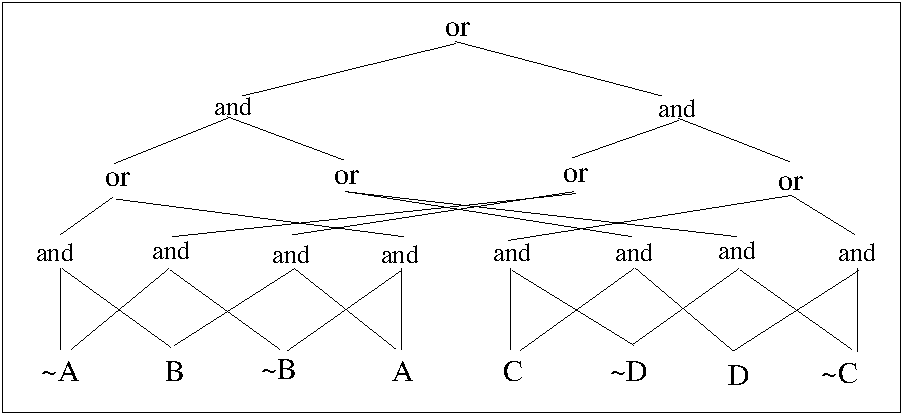
\includegraphics[width=8cm]{odd}
\caption{A decomposable and deterministic NNF.}
\label{fig:dnnf}
\end{figure}


\item[Query Rewriting Solutions] \mbox{}\\
A number of algorithms have been developed to find the rewritings of a given query; the most prominent being the bucket algorithm~\cite{levy:bucket},  the inverse rules algorithm ~\cite{duschka:answer,Qian96}, the minicon algorithm ~\cite{pottinger:minicon}, and the {\it MCDSat} ~\cite{arvelo:aaai06}. Generally, query rewriting algorithms work in two phases: first, they identify the views that rewrite at least one  subgoal of the query; second they combine the selected views to produce a rewriting. The main difference between existing approaches, is the criteria used to choose the relevant views and reduce the space of non-useful rewritings.

The bucket algorithm reduces the number of possibilities just considering each subgoal in the query in isolation, and selecting the views that are able to  produce at least the attributes projected by the query. Since, attributes involved in query joins are not verified, a large number of rewritings comprised of  Cartesian products may  be generated. 	
The Inverse Rules algorithm constructs a set of rules that invert the view definition and establish how to compute tuples for the database relations from tuples of the views. Similarly, to the bucket algorith it can produce a large number non-useful of rewritings. 

The MiniCon algorithm  overcomes the limitations of the previous algorithms by identifying only views that rewrite a set of the query goals and that  can be combined with the rest of the query subgoals. The key idea is to identify the mappings between  the variables in each subgoal of the query to the variables  in one or more subgoals of the views, in a way that, join variables in the query are mapped to join variables in the body of a view or to the distinguished variables of the view. Mappings between variables and subgoals are represented in MiniCon Descriptions (MCD's)\cite{pottinger:minicon}.

Finally,  the
{\it MCDSat} algorithm is able to identify the query rewritings of a query by translating the problem of rewriting
into the problem of enumerating the models of a propositional
theory  $\Theory{\Q}$ whose models are in correspondence
with the rewritings of the query. 
The {\it MCDSat} algorithm exploits the properties of d-DNNFs to efficiently 
compute the MCDs associated with theory $\Theory{\Q}$.
The  {\it MCDSat} algorithm has demonstrated to scale better than the MiniCon
algorithm over a large number of benchmarks often showing performance
improvements of several orders of magnitude. However, the {\it MCDSat} algorithm was not desgined for rewriting problems involving explicit constants,
nor to compute the best rewritings with respect to a given utility function or cost model, and this paper we propose a new encoding  that overcomes these limitations.


\end{description}

\section{The {\it SsdSat} Architecture}
Figure ~\ref{fig:architecture} presents the architecture of{\it SsdSat}; it is comprised of a {\it Catalog} of service descriptions, the {\it SSP Translator},  the {\it c2d}, the {\it Minimal Model Enumerator}, and the {\it Model Translator}.   

\begin{figure}
\centering
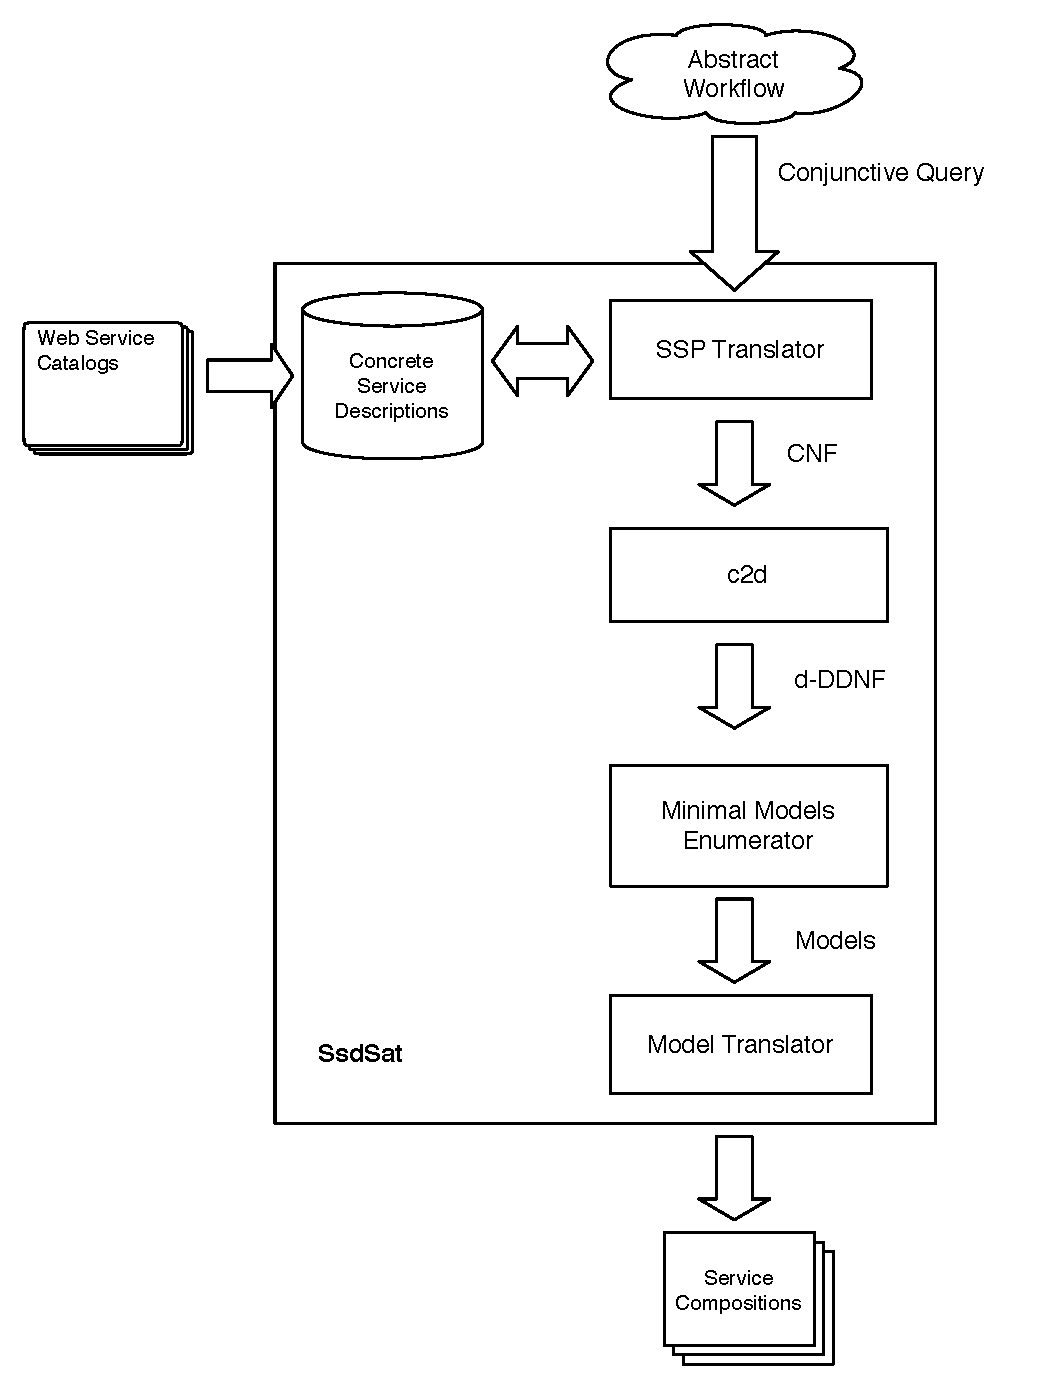
\includegraphics[height=90mm,width=3.5in]{mdcsatC.pdf}
\caption{The {\it SsdSat} Architecture}
\label{fig:architecture}
\end{figure}

First, an instance of the Service Selection Problem is defined as an abstract workflow represented by a conjunctive query on abstract services which is given as input, and a set of concrete services defined by views of abstract services. 

The {\it SsdSat}  Catalog is populated with descriptions of abstract and concrete services; each service is described in terms of input and output attributes of the service, and a real value representing a utility function that aggregates the QoS parameters of the service. Additionally, concrete services are defined as views of abstract services following the paradigm Local As View proposed in ~\cite{levy:bucket}; these descriptions can be generated by the {\cal DEIMOS} system proposed by~\cite{AmbiteISWC09}. 

The {\it SSP Translator} encodes an instance of the Service Selection Problem as a Conjunctive Normal Form formula that corresponds to the propositional logic theory that represents the instance of the problem.  {\it c2d}~\cite{c2d} is an off-the-shell component that compiles  the CNF formula that represents the input instance of the service selection problem into  d-DNNF. {\it c2d} uses conflict direct backtracking with clause learning, and information about the state of clauses to  index into a cache intermediate results. Thus, although the complexity of  compiling CNF into d-DNNF exponentially increases  with the connectivity  of the  CNF, {\it c2d} is able to compile large instances of SSP is few minutes. The {\it Minimal Model Enumerator} extracts the models from  the d-DNNF in linear time; also models counting and enumeration of the model that maximizes the utility function can be performed in linear time. Finally, 
the {\it Model Translator} decodes the models into the service compositions that solve the input problem.





\section{Experimental Results}
We have conducted an empirical analysis  on the benefits of the techniques implemented in the  {\it SsdSat} system.

\begin{description}
\item[Dataset and Query Benchmark:]  we conducted our experiments over a benchmark that includes XX queries and a set of  YY views. Queries and views are starts and chains, and they have between ZZ and TT constants; queries have QQ sub-subgoals.
\item[Evaluation Metrics:] we report on runtime performance which corresponds to the  {\it user time} produced by the {\it time} command of the Unix operation system. 
\end{description}
 
\begin{figure}
\centering
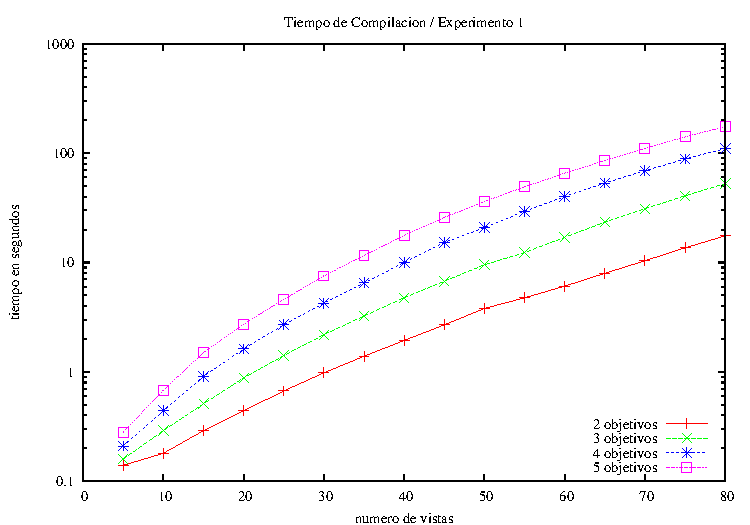
\includegraphics[width=8cm]{plot1.pdf}
\caption{Compilation Time Benchmark I}
\label{fig:plot1}
\end{figure}


\section{Formalization of the Service Selection Problem (SSP)}
We consider service catalogs of the form $C=\tup{S,T}$ where
$S$ is a set of predicates that represent abstract services and $T=\{T_s\}_{s\in S}$ is a collection
of tables that represents the result of the evaluation of the abstract services. In the context of the Service Selection Problem, 
a service catalog $C$ is an idealized description of 
the output produced by abstract workflows  implemented by multiple concrete services described
as views.

A workflow  $Q$ over $S$ is represented by a conjunctive query of the form 
\begin{alignat*}{1}
Q(\vvec{x})\ \qrule\ \  s_1(\vvec{x}_1),\, s_1(\vvec{x}_2),\, \ldots,\, s_m(\vvec{x}_m)\,,
\end{alignat*}
where $s_i\in S$, $\vvec{x}$ is a vector of variables, and each
$\vvec{x}_i$ is a vector of variables and constants.
The result of $Q$ over $C$, denoted as $Q(C)$, is the table with
$|\vvec{x}|$ columns that result of the projection of the relational
join $\join\!\!\{T_{p_i}\}_{i=1}^m$ over $\vvec{x}$.
The atoms in the body of $Q$ are called the (sub)goals of $Q$.

A view $V$ over $C$ is a query over $S$. Given a database $C$, a query $Q$ and a collection of 
views $E=\tup{\{V_i\}_i,\{E_i\}_i}$, we are required to find
all the tuples in $Q(C)$ obtainable from the views in $E$.
That is, we need to find all the \emph{service compositions} of the form
\begin{alignat*}{1}
R(\vvec{x})\ \qrule\ \ V_{i_1}(\vvec{x}_1),\, V_{i_2}(\vvec{x}_2),\, \ldots,\, V_{i_n}(\vvec{x}_n)
\end{alignat*}
such that $R(E) \subseteq Q(C)$.
A service selection problem (SSP) is a tuple $\tup{S,Q,\{V_i\}}$ where $S$
is a set of predicates that represent abstract services, $Q$ is a query over $S$ and $\{V_i\}$ is a collection of views that define the concrete services in terms of  abstract services. We assume \emph{safe} problems in the sense that all 
variables mentioned in the head of the query (resp.\ in the head of each view)
appear in the body of the query (resp.,\ in the body of each view); also the input and output restrictions of the abstract services used in the query are satisfied.
Further, we only deal with SSPs with no arithmetic predicates inside the
query or views.
A service composition $SC$ is \emph{valid} if for all catalogs $C=\tup{S,T}$
and extensions $\{E_i\}$, $R(E) \subseteq Q(C)$.
A collection $\R$ of valid compositions is a solution if
for all service catalogs $C=\tup{S,T}$ and extensions $\{E_i\}$, there
is no other $\R'$ such that $\R(E)\subset\R'(E)\subseteq Q(C)$.
We are interested in finding a service composition $\R$.

\subsection{Logical Theories}
We use an approach similar to one described in ~\cite{arvelo:aaai06} to encode the Service Selection Problem, the reader is referred to \cite{arvelo:aaai06} for a comprehensive
description of the propositional theory. We identify the service compositions by enumerating the
models of a logical theory $\Delta=\Delta_{com}\cup\Delta_{ssd}^1\cup\cdots\Delta_{ssd}^m$
where $\Delta_{com}$ specified how to combine $m$ independent
copies of SSD theories $\Delta_{SSd}$ that cover all goals in $Q$.
Each $\Delta^i_{ssd}$ is a copy of the theory $\Delta_{ssd}$
in which each literal $s$ is tagged as $s^i$.
The theory $\Delta_{ssd}$ consists of different groups of 
clauses that guarantees that its models are in correspondence
with the SSDs, while the theory $\Delta_{com}$ contains additional
clauses to guarantee a sound and complete composition of the SSDs.
A Selection Service Description (SSD) is  $\tup{V,\tau,SS}$ for $\Q$, where $V$ is the concrete service used to cover the subset of abstract services $SS$, and  $\tau\subseteq Vars(Q)\times Vars(V)$ such that all variables in
$\tau_x=\{ y\in Vars(V) : (x,y)\in\tau\}$ are distinguished in $V$. A SSD is a simplification of the MCDs proposed by ~\cite{pottinger:minicon} to characterize the views that can be used to subsets of sub-goals of a query. 

The SSP theory for $\Q$,  denoted by $\Theory{\Q}$, consists
of the following propositional variables:
\begin{enumerate}\denselist
\item $\{v_0,\ldots,v_n\}$ to indicate the SSD uses view $V_i$;
      $v_0$ is used to indicate the \emph{null} SSD,
\item $\{g_1,\ldots,g_m\}$ to indicate the goals in $SS$,
\item $\{z_{j,k,i}\}$ to indicate the $j$th goal in $Q$ is
      covered by the $k$th goal in $V_i$, and
\item $\{t_{x,y}\}$ to indicate that $(x,y)\in\tau$.
\item $t_{x,y}$
to denote that the variable/constant $x$ in the query is mapped
into the variable/constant $y$ in the view, and propositions $v_i$
to indicate that the SSD uses view $V_i$.
\end{enumerate}
The range of indices for the $z$ variables depend on $\Q$;
e.g. if $V_i$ has $K$ goals of the same type as goal
$j$ in $Q$, then $1\leq k\leq K$ for $z_{j,k,i}$.
For $t$ variables, $x$ ranges in the number of variables
in $Q$ and $y$ ranges in the maximum number of variables
in the views.

The following  clauses encode the SSP problem in terms of the SSDs. ~\cite{RajaramanSU95} showed that for queries without negation or arithmetic comparisons,  but with constants, and $m$ goals and $q$ variables, it is enough
to consider service compositions of length at most  $m$ plus  $q$ subgoals ~\cite{Ullman00}.

\begin{enumerate}[C1.]\denselist
\item (At least of view is used): $\bigvee_{i=0}^n v_i$
\item (At most one view is used): $v_i \Rightarrow \neg v_j$ for $0\leq i,j \leq n$,
\item (Null view equals null): $v_0 \Rightarrow \neg g_j$ for $1\leq j\leq m$,
\item (Views are useful): $v_i \Rightarrow \bigvee_{j=1}^m g_j$ for $1\leq i\leq n$,
\item (Subgoals are covered at most once): $z_{j,k,i} \Rightarrow \neg z_{j,l,i}$ for
      appropriate $i,j,k,l$ with $k\neq l$,
\item (Scope of views): $v_i \Rightarrow \neg g_j$ for such goals that can't be covered by $V_i$,
\item (Consistency): $v_i \land g_j \Leftrightarrow \bigvee z_{j,k,i}$ for appropriate $i,j,k$.
\item[C8.] (Dead variables): $v_i \Rightarrow \neg t_{x,y}$ for all $x,y$ with $y\notin V_i$,
\item[C9.] (1-1 for $\exists$ vars): $v_i \land t_{x,y} \Rightarrow \neg t_{x,y'}$ for all
           existential variables $y,y'\in V_i$,
\item[C10.] (Distinguished): $v_i \Rightarrow \neg t_{x,y}$ for all distinguished $x\in Q$ and
            existential $y\in V_i$,
\item[C11.] (Existential): $v_i \land t_{x,y} \Rightarrow g_j$ for all existential $y\in V_i$ and
            goals $j$ that contain $x\in Q$,
\item[C12.] (Matching): $v_i \land z_{j,k,i} \Rightarrow t_{x,y}$ for all $x$ and $y$ that
            should match if goal $j$ in $Q$ is covered by goal $k$ in $V_i$.
\item[C13.] (If all variables in the view are distinguished, then the SSD covers only one goal):
            $v_i \land g_j \Rightarrow \neg g_k$.
\end{enumerate}

These first thirteen are the same clauses used by the {\it MCDSat} to encode the Query Rewriting Problem in propositional logic ~\cite{arvelo:aaai06}. The following clauses are required to allow constants in the workflows and the views. As we showed in Section 2, the main problem when handling constants is to
be sure that different constants are not mapped into each other either directly or indirectly (via transitivity). These clauses ensure that two constants are mapped iff they are the same.

\begin{enumerate}[S1.]\denselist
\item (Inconsistent-1): $t_{x,A} \Rightarrow \neg t_{x,B}$,
\item (Inconsistent-2): $t_{A,x} \Rightarrow \neg t_{B,x}$,
\item (Inconsistent-3): $\neg t_{A,B}$,
\item (Transitivity-1): $v_i\land t_{A,y}\land t_{x,y}\land t_{x,z}\Rightarrow t_{A,z}$,
\item (Transitivity-2): $v_i\land t_{y,A}\land t_{y,x}\land t_{z,x}\Rightarrow t_{z,A}$.
\end{enumerate}
Clauses S1--S3 prune candidate service compositions in which one constant
is directly mapped into a different one, and the last two implement
a restricted propagation of transitivity.
Similarly, $\Delta_{rew}$ must be extended with the clauses:
\begin{enumerate}[S1.]\denselist
\item[S6.] (Inconsistent-4): $t^i_{x,A} \Rightarrow \neg t^j_{x,B}$.
\end{enumerate}

\subsection{Maximum-Utility Function}
We assume a simple additive utility function in which each view
$V_i$ is associated with a utility measure $c(V_i)$, and the overall utility value of
a composition is the sum of the utility values for the views in it.
An optimal or best service composition is one with maximum utility value,
and the optimal utility value of a SSP is the utility value of a best
service composition. A SSP has always a well-defined optimal
utility value (if there are no compositions, its utility is $0$),
but it may have multiple best service compositions.
The service composition problem with utility consists in finding
all the compositions of maximum utility value.
Darwiche \& Marquis \cite{darwiche:weighted} show how to compute the
rank $r^*(\Delta)$ of a propositional theory $\Delta$
efficiently when $r$ is a literal ranking function and
$\Delta$ is in d-DNNF. A literal ranking function ranks
the models of the theory in terms of the rank of the
literals $l$ that are true in the model, and ranks the
theory as the best rank of its models:
\[ r(\omega) = \sum_{\omega\vDash l} r(l),\quad r^*(\Delta) = \max_{\omega\vDash\Delta} r(\omega)\,. \]
Furthermore, not only $r^*(\Delta)$ can be computed
efficiently from the d-DNNF but also the models that
have such rank.
The procedure for computing the rank converts the d-DNNF
into a circuit in which the literals are replaced by their
ranks, the `or' nodes by `max', and the `and' nodes by `sum'.
The evaluation of the circuit computes the rank of $\Delta$.

We thus obtain a simple method for computing the best
rewritings when the literal ranking function $r_c$ induced
by the cost model $c$ is used; $r_c$ is defined by
$r_c(l)=c(V_i)$ if $l=v^t_i$ for some $t$, and $r_c(l)=0$
otherwise.


\section{Conclusions and Future Work}

We have shown how the propositional theory used in {\it MCDSat} can
be extended to support constants, and how it can be used to 
compute the best rewritings with respect to an additive
cost model. The cost model is simple yet expressive.
The computation of the best models relies on an arithmetic
circuit that is obtained from the d-DNNF of the propositional
theory.

\bibliographystyle{abbrv}
\bibliography{ref}

\end{document}
